%!TEX program = xelatex
% rubber: set program xelatex
\documentclass[11pt]{style}

\usepackage{alltt}
\usepackage{longtable}
\usepackage[strict]{chngpage}
\usepackage{acro}

\usepackage{fancyvrb}
\usepackage{hyperref}
\setcounter{tocdepth}{2} % Show only sections in table of contents

\title{OAuth2 \& OpenID}
\def\relator{Poggi Agostino}
\author{Corradi Alessandro}

\graphicspath{{./res/}}

\acsetup{first-style=short}


\begin{document}
\maketitle{}
\pagenumbering{roman}
\tableofcontents
\clearpage


\pagenumbering{arabic}

\subsection{OAuth2}
OAuth2 è uno standard web, utilizzato per fornire token di autorizzazione per risorse protette
a client esterni.

Questi token prendono il nome di \textbf{access token} e lo standard definisce diversi modi per
poterli ottenere.
Ogni modo per ottenere l'access token prende il nome di \textbf{grant type}.

Diversi grant type vengono utilizzati per diversi tipi di applicazioni.
Applicazioni di tipo \textbf{confidential} o confidenziali, sono quelle
che possono salvare con sicurezza delle credenziali.
Un pratico esempio può essere un server web, dove è possibile salvare delle
credenziali in un database o nel codice di backend.

Diversamente, applicazioni mobili o webapp con client-side rendering, rientrano
nella categoria di applicazioni
di tipo \textbf{public} (pubbliche), siccome non hanno modo di salvare una password.


Il tipo di grant più sicuro e raccomandato dalla specifica è quello di tipo \textbf{code},
e richiede un client di tipo confidential.

\subsection{Grant type confidential}
\begin{figure}[h]
    \centering
    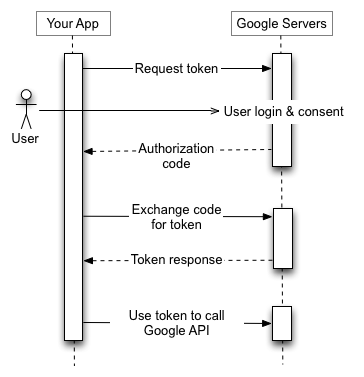
\includegraphics[width=.6\textwidth]{authorization-code.png}
\end{figure}
Prima di effettuare tutti i seguenti step, è necessario registrare
l'applicazione presso il provider di autenticazione, per ottenere delle
credenziali (client id e client secret), necessarie al fine di ottenere
l'access token.
\begin{enumerate}
    \item L'applicazione effettua un redirect sul server di autorizzazione,
        specificando di quali autorizzazioni necessita di essere autorizzato.
    \item L'utente effettua login sul provider di autoizzazione, e sceglie
        se consentire o negare le autorizzazioni richieeste.
    \item In caso di consenso, il provider effettua un redirect contenente nell'url
        un token, chiamato authorization code.
    \item L'applicazione utilizza le sue credenziali ottenute al momento di
        registrazione e l'authorization code, per effettuare una chiamata POST
        verso il provider di autorizzazione.
    \item Il provider autentica l'applicazione e ritorna l'access token.
    \item L'applicazione utilizza l'access token per accedere alle risorse protette.
\end{enumerate}

Il protocollo si basa fortemente su HTTP, TLS e la presenza di un'user-agent.

\subsection{OpenID Connect}
Siccome OAuth2 è un protocollo unicamente per l'autorizzazione, il protocollo
non specifica uno standard con cui riconoscere quale utente sta effettuando
la richiesta utilizzando l'access token.

OpenID connect è un protocollo che estende OAuth2, fornendo la
possiblità di effettuare l'autenticazione attraverso un server dedicato.

Lo standard prevede l'utilizzo di token JWT, crittograficamente firmati e contenenti
informazioni basiche sull'identita dell'utente autenticato.

\subsection{Json Web Token}
I JWT possono essere criptati (JWE), firmati (JWS) o entrambi.
Noi vedremo solo quelli del secondo tipo.

Un JWS è sempre composto da tre sezioni:
\begin{enumerate}
    \item \textbf{head}: contenente metadati riguardanti il JWT, come algoritmo
        utilizzato ed id della chiave crittografica.
\begin{lstlisting}
{'alg': 'RS256', 'kid': '1', 'typ': 'JWT'}
\end{lstlisting}
    \item \textbf{body}: contenente le informazioni vere e propie del JWT, come
        ad esempio l'id dell'utente sul server di autenticazione (\texttt{sub})
\begin{lstlisting}
{'auths': '',
 'iss': 'https://localhost:8000',
 'sub': 2,
 'iat': 1614372435.0381887,
 'exp': 1614376035.0381887}
 \end{lstlisting}
    \item \textbf{signature}: la firma di head e body, concatenati con il carattere ``punto".
\end{enumerate}
\end{document}
% vim: nospell colorcolumn=80
